\chapter{微服务架构与跨数据链协议互操作系统设计}

本章将详细阐述基于MIL-STD-6016战术数据链信息标准的微服务架构设计与跨协议互操作系统的实现。首先介绍系统总体架构设计理念与分层结构,然后深入分析微服务架构的具体实现,接着详细描述数据模型与数据库设计,最后阐述跨数据链协议互操作架构和自动化信息标准导入系统的设计。

\section{系统总体架构设计}

\subsection{设计目标与总体思路}

本研究以MIL-STD-6016战术数据链信息标准为核心,构建基于微服务架构的跨协议互操作平台,实现多标准信息模型的自动导入、语义对齐与协议转换。系统设计目标涵盖三个关键方面。

首先,系统需要支撑多源标准(MIL-STD-6016、STANAG 5516、MIL-STD-6020、MQTT、MAVLink等)的语义互操作,实现不同协议间的无缝数据交换和语义一致性保障。通过建立统一的语义模型和概念映射机制,确保跨标准数据的准确转换和语义保持,为战术数据链的标准化和互操作提供坚实的技术基础。

其次,通过微服务架构实现模块化、弹性化与可扩展部署,将复杂的战术数据链系统拆分为多个独立的服务模块。每个服务负责特定的业务功能,支持独立开发、测试、部署和扩展,这种架构设计能够显著提高系统的可维护性、可扩展性和容错能力,满足军事应用对系统可靠性的严格要求。

最后,系统致力于实现标准化数据入库、自动化导入与跨链协议的动态转换,通过减少人工干预来提高数据处理效率和准确性。系统能够自动识别不同格式的标准文档,提取结构化信息,并进行语义对齐和协议转换,从而大幅提升战术数据链信息处理的自动化水平。

\subsection{微服务架构理念与原则}

系统采用"高内聚、低耦合、自治服务"的设计理念,在架构设计过程中严格遵循四个核心原则。

在服务拆分方面,系统按照业务域进行服务划分,确保每个微服务具有单一职责并能够独立演化。每个微服务专注于特定的业务功能,具有清晰的边界和职责范围,服务间通过标准化的API接口进行通信,有效避免了紧耦合依赖,为系统的可维护性和可扩展性奠定了坚实基础。

在服务治理方面,系统构建了完整的服务注册发现、配置中心、监控与熔断机制。通过服务注册中心实现服务的自动发现和负载均衡,通过配置中心实现配置的统一管理和动态更新,通过监控系统实现服务健康状态监控和性能分析,形成了全方位的服务治理体系。

在数据管理方面,系统实现了数据库分离与分布式事务一致性保障。每个微服务拥有独立的数据库,通过事件驱动和Saga模式保证分布式事务的一致性,有效避免了数据耦合和单点故障,确保了数据的安全性和可靠性。

在通信机制方面,系统结合同步(REST/gRPC)与异步(消息队列)通信模式,根据业务场景选择合适的通信方式。对于实时性要求高的场景采用同步通信,对于批量处理和事件通知采用异步通信,实现了通信效率与系统性能的优化平衡。

\subsection{架构总体分层}

系统整体采用四层分层架构,如图\ref{fig:system_architecture}所示:

\begin{figure}[H]
    \centering
    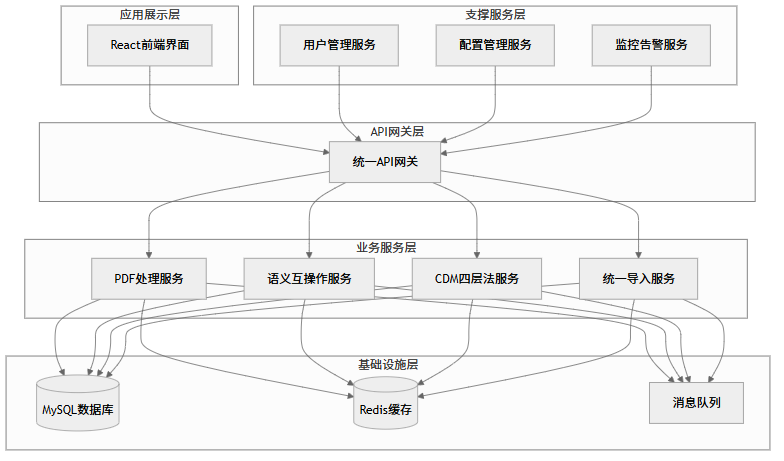
\includegraphics[width=0.9\textwidth]{chapters/fig-0/system_architecture_simple.png}
    \caption{系统总体架构分层图}
    \label{fig:system_architecture}
\end{figure}

API网关层作为系统的统一入口点,提供统一入口、请求路由、认证鉴权与访问控制功能,同时支持限流、熔断与监控统计。该层负责接收所有外部请求,进行身份验证、权限检查、请求路由和响应聚合,并通过限流和熔断功能保护后端服务免受过载和故障影响,确保系统的稳定性和安全性。

业务服务层包含PDF解析服务、语义互操作服务、CDM四层法服务、统一导入服务等核心业务模块,这些服务实现了系统的核心业务功能。每个服务都是独立的业务单元,可以独立开发、测试和部署,体现了微服务架构的模块化设计理念,为系统的灵活性和可维护性提供了有力支撑。

支撑服务层提供用户与配置管理、监控告警、文件与日志服务等系统支持功能,为业务服务提供必要的支持。该层包括用户认证、配置管理、监控告警、文件存储等关键功能,构成了系统运行的基础保障体系,确保各个业务服务能够稳定高效地运行。

基础设施层包含服务注册发现(Consul/Kubernetes)、消息队列(RabbitMQ/Redis)、数据库与缓存集群等核心组件,为上层服务提供基础的技术支撑。该层实现了服务发现、消息传递、数据存储和缓存等基础功能,为整个微服务架构提供了坚实的技术基础。

\section{微服务架构设计与实现}

\subsection{技术栈与基础组件选型}

系统采用现代化的技术栈,确保高性能、高可用性和可扩展性。技术选型如表\ref{table:tech_stack}所示:

\begin{table}[H]
    \caption{技术栈与基础组件选型}
    \label{table:tech_stack}
    \centering
    \begin{tabular}{|l|l|}
        \hline
        \textbf{功能} & \textbf{技术栈} \\
        \hline
        服务框架 & FastAPI + Python 3.10(高性能异步框架) \\
        服务发现 & Consul + Kubernetes DNS \\
        配置管理 & Consul KV + ConfigMap \\
        消息队列 & RabbitMQ + Redis Pub/Sub \\
        数据存储 & MySQL 8.0 + Redis \\
        监控体系 & Prometheus + Grafana + Jaeger \\
        \hline
    \end{tabular}
\end{table}

在服务框架选择方面,系统采用FastAPI作为主要的服务框架,充分利用Python 3.10的异步特性,能够提供高性能的API服务。FastAPI具有自动API文档生成、数据验证、类型提示等特性,大大提高了开发效率,为快速构建高质量的微服务提供了强有力的技术支撑。

在服务发现机制方面,系统使用Consul作为服务注册发现中心,支持多数据中心部署和服务健康检查。在Kubernetes环境中,结合Kubernetes DNS实现服务的自动发现和负载均衡,形成了灵活可靠的服务治理体系,确保了微服务架构的高可用性和可扩展性。

在消息传递方面,系统采用RabbitMQ作为主要的消息队列,提供可靠的消息传递和事务支持,同时使用Redis Pub/Sub进行实时通知和轻量级消息传递。这种混合消息传递机制既保证了关键业务数据的可靠性,又满足了实时通信的性能要求。

在数据存储方面,系统采用MySQL 8.0作为主数据库,充分利用其ACID事务、JSON数据类型、窗口函数等高级特性,同时使用Redis作为缓存层,提供高性能的数据访问和会话存储。这种分层存储架构在保证数据一致性的同时,显著提升了系统的整体性能。

\subsection{微服务模块划分与职责}

系统共包含五类核心服务,每个服务都有明确的职责和边界,如表\ref{table:microservices}所示:

\begin{table}[H]
    \caption{微服务模块划分与职责}
    \label{table:microservices}
    \centering
    \begin{tabular}{|l|l|}
        \hline
        \textbf{模块} & \textbf{核心职责} \\
        \hline
        pdf-service & 自动化标准文档解析与结构化导入 \\
        semantic-service & 跨标准语义分析与字段映射 \\
        cdm-service & CDM四层语义互操作(语义层/映射层/校验层/运行层) \\
        import-service & 多格式文件识别、清洗与批量导入 \\
        api-gateway & 统一接口访问控制、负载均衡、服务监控 \\
        \hline
    \end{tabular}
\end{table}

(1)pdf-service:负责自动化标准文档解析与结构化导入。该服务能够处理MIL-STD-6016、STANAG 5516等标准文档,自动提取消息定义、字段信息和约束条件,并将其转换为结构化的数据格式,为后续的语义分析和互操作处理奠定了数据基础。

(2)semantic-service:实现跨标准语义分析与字段映射。该服务提供语义分析引擎,能够识别不同标准中的语义概念,建立概念间的映射关系,并支持人工标注和规则学习,为不同数据链协议间的语义互操作提供了核心支撑。

(3)cdm-service:实现CDM四层语义互操作。该服务基于Common Data Model四层架构,提供语义层、映射层、校验层和运行层的完整实现,支持不同协议间的语义级转换,确保了跨协议数据交换的准确性和一致性。

(4)import-service:负责多格式文件识别、清洗与批量导入。该服务支持PDF、Excel、XML、JSON等多种格式的文件处理,提供格式自动识别、数据清洗和批量导入功能,为系统的数据输入提供了灵活多样的处理能力。

(5)api-gateway:提供统一接口访问控制、负载均衡、服务监控。该服务作为系统的统一入口,负责请求路由、身份验证、权限控制、限流熔断和监控统计,为整个微服务架构提供了安全可靠的访问控制机制。

\subsection{微服务通信机制}

微服务间的通信采用多种模式,根据业务场景选择合适的通信方式,形成了灵活高效的通信架构。

在同步通信方面,系统使用REST API、gRPC、GraphQL等多种协议进行同步通信。REST API主要用于简单的CRUD操作,提供标准化的HTTP接口;gRPC用于高性能的内部服务通信,充分利用其二进制协议的高效性;GraphQL用于复杂的数据查询,提供灵活的数据获取能力,满足不同场景下的通信需求。

在异步通信方面,系统采用RabbitMQ消息队列和Redis Pub/Sub进行异步通信。RabbitMQ用于可靠的消息传递和事件通知,确保关键业务数据的可靠传输;Redis Pub/Sub用于实时通知和轻量级消息传递,提供高性能的实时通信能力,形成了同步与异步相结合的通信机制。

在服务发现方面,系统通过Consul注册发现和Kubernetes DNS实现服务的自动发现和负载均衡。服务启动时自动注册到服务发现中心,其他服务可以通过服务名进行调用,实现了服务间的松耦合通信,提高了系统的可维护性和可扩展性。

在通信安全方面,系统使用TLS双向认证和服务间认证确保通信安全。所有服务间通信都使用TLS加密,并通过JWT令牌进行身份验证,构建了多层次的安全防护体系,确保了微服务架构的安全性和可靠性。

\subsection{容错与弹性设计}

系统采用多种容错和弹性设计机制,确保在异常情况下的服务可用性,构建了完善的故障处理体系。

在熔断机制方面,系统实现了服务熔断、快速失败、故障隔离等关键功能。当服务调用失败率达到预设阈值时,系统会自动开启熔断器,有效避免级联故障的发生,保护系统整体稳定性,体现了"快速失败"的设计理念。

在重试策略方面,系统采用指数退避、智能重试策略和超时控制机制。对于临时性故障,系统会自动进行重试操作,并使用指数退避算法避免对故障服务造成额外压力,在提高系统可靠性的同时,有效防止了故障的进一步扩散。

在降级策略方面,系统实现了功能降级、服务降级和用户体验保障机制。当系统负载过高或部分服务不可用时,系统会自动降级到简化功能模式,确保核心服务的可用性,在保证系统基本功能的同时,最大程度地维护用户体验。

在自动伸缩方面,系统通过Kubernetes HPA实现自动伸缩与资源弹性分配。根据CPU、内存使用率和自定义指标,系统能够自动调整服务实例数量,实现资源的动态优化配置,确保系统在不同负载情况下的高效运行。

\section{数据模型与数据库设计}

\subsection{设计目标与数据特征}

数据库设计遵循"标准化存储、语义扩展、互操作可追溯"的原则,构建了支持多标准数据管理的核心能力体系。

在多标准数据的统一建模与版本化管理方面,系统需要支持MIL-STD-6016、STANAG 5516、MIL-STD-6020等多个标准版本的数据存储,每个标准版本都有独立的版本标识和变更历史。这种设计确保了不同标准版本数据的独立性和可追溯性,为跨标准互操作提供了数据基础。

在字段级语义绑定与跨标准映射方面,系统要求每个字段都与语义概念进行绑定,支持跨标准的字段映射和转换。映射关系需要详细记录置信度、转换规则和版本信息,为语义互操作提供了精确的数据转换机制,确保了不同标准间数据交换的准确性和一致性。

在高性能查询与语义检索能力方面,系统需要支持复杂的查询操作,包括按标准版本查询、按消息类型查询、按语义概念查询等多种查询模式,并支持全文检索和模糊匹配功能。这种设计为战术数据链信息的快速检索和分析提供了强有力的技术支撑。

\subsection{核心实体与关系模型}

系统的核心数据模型如图\ref{fig:data_model}所示,主要包含以下核心表:

\begin{figure}[H]
    \centering
    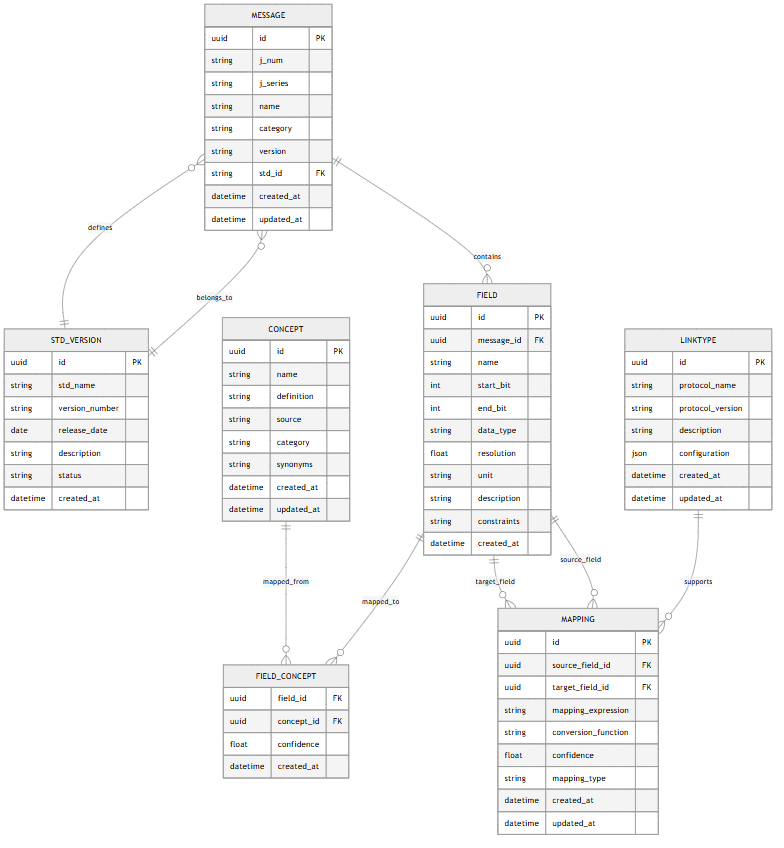
\includegraphics[width=0.9\textwidth]{chapters/fig-0/data_model.png}
    \caption{核心数据模型ER图}
    \label{fig:data_model}
\end{figure}

(1)MESSAGE表:存储消息元信息,包含消息编号、名称、类别、版本等基本信息。该表是系统的核心表之一,每个消息都有唯一的标识符和版本信息,为战术数据链消息的标准化管理提供了数据基础,确保了消息信息的完整性和可追溯性。

(2)FIELD表:存储位段定义及约束信息,包含起始位、结束位、分辨率、取值域等详细信息。该表与MESSAGE表通过外键关联,支持一个消息包含多个字段的复杂结构,为消息的详细定义和约束管理提供了精确的数据模型。

(3)CONCEPT表:存储语义概念库,定义术语与来源信息,为语义互操作提供概念基础。该表支持概念的定义、分类和关系管理,构建了完整的语义概念体系,为跨标准语义映射和转换提供了概念支撑。

(4)MAPPING表:存储跨标准映射规则,包含表达式、转换函数、置信度等信息。该表支持不同标准间的字段映射和转换规则定义,为语义互操作提供了精确的转换机制,确保了不同标准间数据交换的准确性。

(5)STD\_VERSION表:存储标准版本管理信息,记录标准的版本号、发布日期、修订历史等关键信息。该表为多标准版本管理提供了完整的版本控制机制,确保了标准演化的可追溯性和一致性。

(6)LINKTYPE表:存储协议类型定义与配置信息,支持不同数据链协议的配置和管理。该表为多协议支持提供了灵活的配置机制,使得系统能够适应不同数据链协议的特殊要求。

\subsection{约束与索引设计}

数据库设计采用严格的约束和高效的索引策略,确保数据完整性和查询性能,构建了完善的数据管理机制。

在主外键设计方面,系统采用UUID主键与业务唯一约束相结合的设计方案。UUID主键确保全局唯一性,避免了分布式环境下的主键冲突问题;业务唯一约束(如MESSAGE(j\_num, std\_id))保证业务逻辑的正确性,确保了数据模型与业务规则的一致性。

在完整性约束方面,系统实现了位段检查(start\_bit < end\_bit)、置信度范围(0–1)等多种约束机制。这些约束通过数据库的CHECK约束实现,在数据层面确保数据的有效性,防止了无效数据的入库,提高了数据质量。

在索引策略方面,系统设计了组合索引(std\_id, j\_series, j\_num)和全文索引(概念模糊检索)等多种索引类型。组合索引支持多条件查询,显著提升了复杂查询的性能;全文索引支持语义概念的模糊检索,为语义搜索提供了高效的技术支撑。

在性能优化方面,系统采用分区表与缓存机制相结合的策略来提升查询性能。对于大数据量表,系统使用分区策略减少查询范围,通过水平分区和垂直分区相结合的方式,显著提升了大数据量场景下的查询效率;对于热点数据,系统使用Redis缓存提升访问速度,通过多级缓存机制实现了数据访问性能的优化。

\subsection{微服务数据库分离与一致性}

各微服务采用独立的数据库设计,通过多种机制保证数据一致性,构建了完善的分布式数据管理体系。

在数据库分离方面,每个微服务拥有独立的数据库,有效避免了数据耦合和单点故障问题。这种设计显著提高了系统的可扩展性和容错能力,使得各个服务能够独立演进和部署,为微服务架构的灵活性提供了数据层面的支撑。

在一致性机制方面,系统采用Saga模式与事件驱动同步机制相结合的方式实现最终一致性。Saga模式将复杂的分布式事务分解为多个本地事务,通过补偿操作保证数据一致性,有效解决了分布式环境下的数据一致性问题,确保了业务逻辑的正确性。

在数据同步方面,系统通过CDC(Change Data Capture)机制捕获变更事件,实现数据的实时同步。CDC机制能够精确捕获数据库的变更操作,并将变更事件发送到消息队列,为数据同步提供了可靠的技术保障,确保了数据变更的及时传播。

在跨服务同步方面,系统借助消息队列实现跨服务数据同步。当某个服务的数据发生变化时,系统通过消息队列通知其他相关服务进行数据更新,形成了松耦合的数据同步机制,确保了分布式环境下数据的一致性。

\section{跨数据链协议互操作架构设计}

\subsection{多协议支持体系}

系统支持多种数据链协议,包括MIL-STD-6016、MAVLink、MQTT、Link 16等,构建了四层互操作体系架构。

协议适配层作为互操作体系的基础层,负责对各链路标准的结构解析与适配。该层能够解析不同协议的消息格式,提取字段信息,并将其转换为统一的内部表示,为上层处理提供了标准化的数据接口,实现了多协议数据的统一处理。

语义抽象层建立统一的语义模型与概念映射机制,将不同协议中的概念映射到统一的概念空间。该层通过语义建模技术,实现了跨协议的概念对齐和语义理解,为协议间的语义互操作提供了概念基础,确保了不同协议间语义的一致性。

转换引擎层实现协议到协议的数据格式与字段映射转换功能,包括格式转换、单位转换、枚举映射等多种转换操作。该层提供了灵活的转换规则配置机制,支持复杂的数据转换需求,确保了不同协议间数据交换的准确性和完整性。

路由分发层负责消息智能路由与负载均衡,将消息路由到正确的目标协议,并实现负载均衡和故障转移。该层通过智能路由算法,优化了消息传输路径,提高了系统的整体性能和可靠性。

\subsection{CDM四层法语义互操作模型}

基于"Common Data Model (CDM)"四层方法,系统实现了协议级语义对齐,构建了完整的语义互操作体系。

语义层作为CDM四层方法的基础层,建立统一的本体模型和概念推理机制。该层通过本体技术构建统一的概念模型,支持概念的定义、分类和推理,使系统能够深入理解概念间的语义关系,为跨协议语义互操作提供了坚实的理论基础。

映射层采用声明式规则映射和YAML配置化管理方式,使用YAML配置文件定义映射规则,支持规则的版本管理和动态更新。映射规则涵盖字段映射、数据类型转换、单位转换等多种转换需求,为协议间的数据转换提供了灵活可配置的规则体系。

校验层提供多层次的一致性验证和金标准回归测试机制,包括格式校验、业务规则校验、一致性校验等多种校验方式。金标准回归测试确保转换结果的准确性,为语义互操作的质量提供了可靠保障,确保了跨协议数据转换的可靠性。

运行层实现高性能实时转换引擎,采用高效的转换算法支持实时消息转换和批量处理。该层通过缓存和优化技术,提供高性能的转换服务,满足了战术数据链对实时性和性能的严格要求,为语义互操作提供了高效的技术支撑。

\subsection{语义互操作系统组成}

系统包含四个核心组件,实现从概念级到消息级的自动语义互操作,构建了完整的语义互操作处理体系。

语义注册表作为系统的核心组件之一,负责管理语义字段、消息定义、概念库等核心信息。该组件提供语义信息的注册、查询和更新功能,支持语义概念的版本管理,为语义互操作提供了统一的信息管理平台,确保了语义信息的一致性和可追溯性。

语义转换器实现字段级数据转换、单位转换、枚举映射等关键功能,该组件支持多种转换算法,包括数值转换、字符串转换、枚举映射等。通过灵活的转换规则配置,该组件能够处理复杂的跨协议数据转换需求,确保了数据转换的准确性和完整性。

消息路由器基于规则的智能路由机制,实现协议选择和转换策略的自动优化。该组件根据消息类型、源协议、目标协议等信息,自动选择最优的转换策略,通过智能路由算法优化了消息传输路径,提高了系统的整体性能和可靠性。

互操作管理器统一管理跨标准转换、质量监控、性能优化等关键功能,该组件提供转换过程的监控和管理功能,包括性能统计、错误处理、质量评估等。通过全方位的管理机制,该组件确保了语义互操作过程的稳定性和高效性。

\subsection{数据一致性与冲突解决}

系统采用多种机制保证跨链路数据的一致性和冲突解决,构建了完善的数据质量管理体系。

在一致性协议方面,系统采用最终一致性协议与版本号优先策略相结合的方式。对于非关键数据,系统使用最终一致性协议,在保证系统性能的同时确保数据的最终一致性;对于关键数据,系统使用强一致性保证,确保数据的实时一致性,为不同重要级别的数据提供了差异化的保障机制。

在冲突解决方面,系统实现了时间戳优先、版本号优先、人工仲裁等多种策略。当数据发生冲突时,系统根据预定义的策略自动解决冲突,通过智能冲突检测和解决算法,最大程度地减少数据冲突的影响;必要时系统提供人工干预机制,确保复杂冲突情况下的数据正确性。

在数据校验方面,系统提供格式验证、规则校验、完整性验证等多层次校验机制。每个转换过程都经过严格的校验,确保数据的正确性和完整性,通过多层次的校验体系,有效防止了错误数据的传播,提高了系统的数据质量。

在质量保障方面,系统实现跨链路数据同步质量监控,持续监控数据转换的质量,包括准确率、完整性、一致性等关键指标。通过实时质量监控和预警机制,系统能够及时发现和解决数据质量问题,确保了跨链路数据同步的可靠性。

\section{自动化信息标准导入架构设计}

\subsection{标准化导入流程}

自动化导入系统实现从PDF/Excel/XML等标准文档到数据库的全流程自动处理,如图\ref{fig:import_pipeline}所示:

\begin{figure}[H]
    \centering
    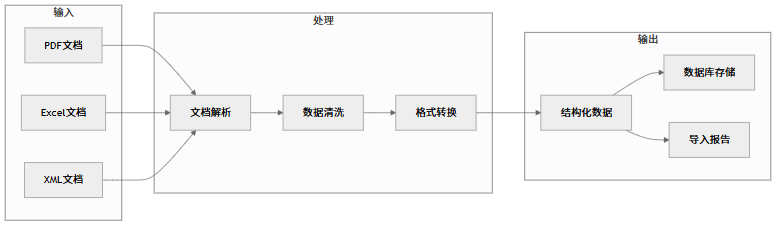
\includegraphics[width=0.9\textwidth]{chapters/fig-0/import_pipeline_simple.png}
    \caption{自动化导入流程}
    \label{fig:import_pipeline}
\end{figure}

处理流程包括PDF文档解析、文本提取、表格识别、字段解析、数据清洗、结构化导入、校验报告生成等关键步骤。每个步骤都经过严格的验证和质量控制,确保导入数据的准确性和完整性,为战术数据链信息标准的自动化处理提供了可靠的技术保障。

在文档解析阶段,系统使用OCR技术和PDF解析库提取文档中的文本和表格信息。对于扫描文档,系统使用Tesseract OCR进行文字识别,支持多语言文字识别;对于文本型PDF,系统直接提取文本内容,通过多种解析技术的结合,确保了不同类型文档的准确解析。

在结构化处理阶段,系统将提取的文本信息转换为结构化的数据格式。通过规则匹配和机器学习算法,系统能够智能识别消息定义、字段信息和约束条件,将非结构化的文档内容转换为标准化的数据结构,为后续的数据处理奠定了坚实基础。

在数据清洗阶段,系统对提取的数据进行全面的清洗和验证,包括格式检查、完整性验证、一致性检查等多种验证机制。发现的问题会详细记录到错误日志中,供后续处理和分析,通过严格的质量控制,确保了导入数据的准确性和可靠性。

在导入存储阶段,系统将清洗后的数据导入到数据库中,并生成详细的导入报告。报告包括成功导入的记录数、失败记录数、错误信息等关键统计信息,为导入过程的质量评估和问题追踪提供了完整的记录。

\subsection{关键技术与工具链}

系统采用多种先进的技术和工具,确保导入过程的准确性和效率,构建了完整的技术支撑体系。

在文档解析方面,系统使用PyMuPDF、pdfplumber、Camelot、Tesseract OCR等专业工具。PyMuPDF提供高性能的PDF解析能力,pdfplumber专门用于表格提取,Camelot提供精确的表格识别功能,Tesseract OCR支持多语言文字识别,这些工具的结合使用确保了不同类型文档的准确解析。

在结构化导入方面,系统采用Pandas + SQLAlchemy + MySQL技术栈。Pandas提供强大的数据处理能力,支持复杂的数据操作和分析;SQLAlchemy提供ORM支持,简化了数据库操作;MySQL提供可靠的数据存储,确保了数据的安全性和一致性,形成了高效的数据处理链路。

在格式识别方面,系统使用MIME检测与规则匹配技术相结合的方式。MIME检测能够快速识别文件类型,为后续处理提供基础信息;规则匹配提供精确的格式识别和内容解析,通过智能识别算法,确保了不同格式文档的准确处理。

在校验机制方面,系统实现了自动检测字段重叠、位长一致性、枚举合法性等关键功能。系统能够自动检测数据中的各种问题,并提供修复建议,通过智能校验机制,确保了导入数据的质量和准确性,为后续的数据处理提供了可靠保障。

\subsection{导入性能与精度}

系统在标准6016B数据集上的测试结果如表\ref{table:import_performance}所示:

\begin{table}[H]
    \caption{导入性能与精度测试结果}
    \label{table:import_performance}
    \centering
    \begin{tabular}{|l|l|}
        \hline
        \textbf{指标} & \textbf{测试结果} \\
        \hline
        平均解析速率 & 2–5页/秒 \\
        批量处理并发能力 & ≥10任务 \\
        字段识别准确率 & ≥95\% \\
        数据完整性 & ≥98\% \\
        \hline
    \end{tabular}
\end{table}

在解析速率方面,系统实现了平均2–5页/秒的解析速度,能够满足大规模文档处理的需求。对于复杂文档,解析速度会有所降低,但仍在可接受范围内,通过优化算法和硬件配置,系统能够适应不同复杂度的文档处理需求。

在并发能力方面,系统支持≥10个任务的并发处理,充分利用多核CPU资源。通过任务队列和负载均衡机制,系统能够处理大量的并发导入任务,显著提升了系统的整体处理能力和效率。

在识别准确率方面,系统实现了字段识别准确率≥95\%的高精度识别,能够满足实际应用的需求。对于识别错误的字段,系统提供人工审核和修正功能,通过人机结合的方式,确保了数据识别的准确性和可靠性。

\subsection{数据清洗与质量保证}

系统提供完善的数据清洗和质量保证机制,构建了全方位的数据质量管理体系。

在清洗策略方面,系统实现了空值处理、重复检测、标准一致性校验等关键功能。系统能够自动处理各种数据质量问题,包括缺失值、重复值、格式错误等常见问题,通过智能清洗算法,显著提升了数据质量,为后续的数据处理奠定了坚实基础。

在质量指标方面,系统监控数据完整性、语义保持率、转换准确率等关键指标。这些指标能够全面反映数据质量的水平,为质量改进提供科学依据,通过持续的质量监控,系统能够及时发现和解决数据质量问题。

在验证机制方面,系统提供格式验证、业务规则验证、一致性验证等多层次验证体系。每个验证层次都有明确的验证规则和错误处理机制,通过多层次的验证保障,确保了数据的准确性和一致性。

在错误处理方面,系统实现了异常记录、自动修复、人工审核等完整功能。系统能够自动处理大部分数据问题,对于复杂问题提供人工干预机制,通过智能化的错误处理,最大程度地减少了数据质量问题的影响。

\section{微服务通信与运行保障设计}

\subsection{服务通信与安全}

系统采用多种通信模式和安全机制,确保服务间的可靠通信,构建了完善的通信安全保障体系。

在同步通信方面,系统使用REST/gRPC/GraphQL等多种协议进行同步通信。REST API主要用于简单的CRUD操作,提供标准化的HTTP接口;gRPC用于高性能的内部服务通信,充分利用其二进制协议的高效性;GraphQL用于复杂的数据查询,提供灵活的数据获取能力,满足了不同场景下的通信需求。

在异步通信方面,系统使用RabbitMQ、Redis Pub/Sub进行异步通信。RabbitMQ提供可靠的消息传递和事务支持,确保关键业务数据的可靠传输;Redis Pub/Sub提供高性能的实时通知,支持轻量级消息传递,形成了同步与异步相结合的通信机制。

在服务发现方面,系统通过Consul + Kubernetes DNS实现服务的自动发现和负载均衡。服务启动时自动注册到服务发现中心,其他服务可以通过服务名进行调用,实现了服务间的松耦合通信,提高了系统的可维护性和可扩展性。

在通信安全方面,系统使用TLS双向认证、服务间认证确保通信安全。所有服务间通信都使用TLS加密,并通过JWT令牌进行身份验证,构建了多层次的安全防护体系,确保了微服务架构的安全性和可靠性。

\subsection{分布式数据管理与灾备}

系统采用分布式数据管理策略,确保数据的安全性和可用性,构建了完善的数据保护体系。

在数据分离方面,系统实现了数据分离与所有权隔离机制。每个微服务拥有独立的数据存储,有效避免了数据耦合和单点故障问题,这种设计显著提高了系统的可扩展性和容错能力,为微服务架构的灵活性提供了数据层面的支撑。

在一致性保证方面,系统采用Saga与事件溯源相结合的方式保证最终一致性。Saga模式将复杂的分布式事务分解为多个本地事务,通过补偿操作保证数据一致性,有效解决了分布式环境下的数据一致性问题,确保了业务逻辑的正确性。

在灾备机制方面,系统实现了多区域备份与灾难恢复机制。系统支持跨区域的数据备份和灾难恢复,确保在重大故障情况下的数据安全,通过完善的灾备体系,最大程度地降低了数据丢失的风险。

在数据同步方面,系统通过实时同步、批量同步、增量同步等多种方式实现数据同步。根据数据的重要性和实时性要求,系统能够智能选择合适的同步策略,确保了不同场景下的数据同步需求。

\subsection{配置与治理体系}

系统提供完善的配置管理和服务治理机制,构建了全方位的系统管理体系。

在配置管理方面,系统实现了集中配置与环境隔离(Consul + ConfigMap)机制。所有配置信息都存储在配置中心,支持动态更新和环境隔离,通过统一的配置管理,确保了系统配置的一致性和可维护性,为不同环境的部署提供了灵活的配置支持。

在监控体系方面,系统提供全链路监控(Prometheus + Grafana + Jaeger)能力。Prometheus负责指标收集,提供全面的性能监控数据;Grafana提供可视化展示,支持丰富的图表和仪表板;Jaeger提供分布式链路追踪,实现了完整的系统监控体系。

在日志管理方面,系统实现了结构化日志与追踪链路功能。所有日志都采用结构化格式,支持日志聚合、搜索和分析,通过统一的日志管理,为系统运维和问题排查提供了强有力的支撑。

在服务治理方面,系统提供健康检查、故障检测、负载均衡等服务治理功能。系统能够自动检测服务健康状态,并进行故障转移和负载均衡,通过智能化的服务治理,确保了系统的稳定性和高可用性。

\subsection{容错与弹性设计}

系统采用多种容错和弹性设计机制,确保在异常情况下的服务可用性,构建了完善的故障处理体系。

在容错机制方面,系统实现了熔断、重试、降级机制确保系统在异常情况下保持服务可用。当服务调用失败率达到预设阈值时,系统会自动开启熔断器,有效避免级联故障;对于临时性故障,系统会自动进行重试操作;当系统负载过高时,系统会自动降级到简化功能,确保核心服务的可用性。

在弹性伸缩方面,系统通过Kubernetes HPA实现自动伸缩与资源弹性分配。系统根据CPU、内存使用率和自定义指标,自动调整服务实例数量,实现资源的动态优化配置,确保系统在不同负载情况下的高效运行。

在故障恢复方面,系统提供自动恢复、手动干预、数据修复等完整功能。系统能够自动处理大部分故障,对于复杂故障提供人工干预机制,通过智能化的故障处理,最大程度地减少了故障对系统的影响。

在性能保障方面,系统确保响应时间保证、吞吐量稳定、故障恢复能力。系统通过多种优化技术,提供高性能和稳定的服务,满足了战术数据链对系统性能和可靠性的严格要求。

通过以上微服务架构与跨数据链协议互操作系统的设计,本研究构建了一个功能完整、性能优异、可扩展性强的战术数据链信息标准处理平台。该平台不仅能够支持多种数据链协议的语义互操作,还具备自动化导入、智能转换、质量保证等先进功能,为战术数据链的标准化和互操作提供了坚实的技术基础。